\documentclass[11pt, letterpaper]{article}
\usepackage[utf8]{inputenc}
\title{Medical Assistent}
\author{Adrian Locher, Jason Benz}
\date{\today}

\usepackage{graphicx}

\begin{document}
\pagenumbering{gobble}
\maketitle

\newpage
\tableofcontents
\newpage

\pagenumbering{arabic}

\section{Einleitung}
    \subsection{Motivation}
        \paragraph{}
            Die Frage, ob ein Arzt besucht werden soll, ist häufig ein Dilemma.
            Einerseits, will man nicht diejenige Person sein, welche bei unbedenklichen Symptomen
            überreagiert, andererseits könnten sich die Symptome ja verschlimmern und vielleicht
            hätte der Arztbesuch das Problem frühzeitig beheben können. Aus solchen Gründen ist man ja
            schliesslich versichert.

        \paragraph{}
            Eine ganz andere Beudeutung hat dieses Dilemma ausserdem seit dem Anfang
            der Covid-19 Situation. Ärzte und anderes Gesundheitspersonal, gelten als besonders
            stark ausgelastet. Auf der kehrseite hingegen, sollte man bei Covid-19-artigen Symptomen
            auch nicht zögern und sich testen lassen. Welche Symptome nun genau als "Covid-Symptome"
            gelten und welche nicht, ist teilweise sehr unübersichtlich, was die lage auch nicht
            einfacher werden lässt.

        \paragraph{}
            Das Ziel unseres Projekts, soll sein eine lösung zu entwickeln, mit der unnötige Arztbesuche
            generell, aber besonders in Situationen wie jetzt vermieden werden können.
            Das Ziel ist nicht, dass einfach grundsätzlich weniger Menschen Arztbesuche machen, sondern
            vielmehr, in Grenzfällen bei der Entscheidung zu helfen.
        
        \paragraph{}
            Um dabei auch wirklich das Gesundheitspersonal maximal zu entlasten, besteht unser
            Lösungsansatz nicht etwa aus einer Hotline. Ziel ist es ein AI gestützes System zu entwickeln,
            welches ganz ohne Menschliche Interaktion auf seiten der Gesundheitsbranche auskommt.

\newpage

\section{Java Client}

\newpage

\section{Backend}
    \subsection{Übersicht}
        \paragraph{}
            Das Backend ist in 4 Intents strukturiert
            \begin{figure}[h!]
                \begin{center}
                    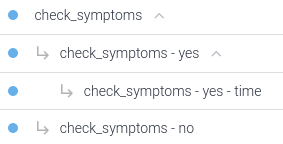
\includegraphics[width=0.5\linewidth]{ressources/intents.png}
                \end{center}
                \caption{Dialogflow intent liste}
                \label{fig:intentslist}
            \end{figure}
    \subsection{Aufnahme von Symptomen}
        \paragraph{}
            Im ersten Intent, des Dialogs - "check\_symtpoms" - wird eine Liste an
            symptomen, sowie ein Schmerzniveau und die Zeitdauer, seit dem die Symptome
            bestehen aufgenommen.

        \paragraph{}
            Folgende Trainingssätze, wurden für das Auslösen des Intents definiert:
            \begin{itemize}
                \item i have \emph{pain} since \emph{yesterday}
                \item i have \emph{pain}
                \item i need help
                \item should i go to the doctor?
                \item Can you tell me if i should seee a doctor?
                \item Am I sick?
                \item I feel Sick
                \item feel \emph{unwell}
            \end{itemize}
            Wobei, hier \emph{kursiv} geschrieben Wörter auf entsprechende Parameter gematcht wurden.

        \subsubsection{Parameter Entities}
            Um die Symptom-Parameter aufzuzeichnen wurden folgende Parameter und Entities definiert:
            \begin{table}[!h]
                \begin{center}
                    \begin{tabular}{c|c}
                        \textbf{Parameter} & \textbf{Entity}\\
                        \hline
                        SymType & symptom\_type\\
                        SymIntensity & symtom\_intensity\\
                        SymDuration & System.Date
                    \end{tabular}
                    \caption{Paramter und Entities}
                    \label{tab:tabelleParamsUndEntities}
                \end{center}
            \end{table}
            
            \paragraph{}
                \textbf{symtom\_type} hat einen Wertebereich von: pain, unwell,
                sick, fever, cough, loss of taste, chestpain, tiredness \& shortness of breath. Mit jeweils 3 bis 4 
                Synonymoen.
            
            \paragraph{}
                \textbf{symtom\_intensity} hat einen Wertebereich von 1 bis 5 jeweils Wörtltlich (z.B. "One", "Eins") und
                Buchstäblich (z.B. 1).
            
            \paragraph{}
                \textbf{Sys.Date} ist ein vorgefertigtes Entity mit einem Wertebereich, welcher beliebige Kelanderdaten
                enthalten kann.
    \subsection{Auswertung der Symptome}
        \paragraph{}
            In einem zweiten Schritt geht es nun darum die Angaben auszuwerten, damit dem Patienten tipps, zu weiterem verhalten
            gegeben werden können. Die Auswertung findet am ende des Intents statt, indem ein Webhook aufgerufen wird.
            Hier ist als Antwort auf den entsprechenden Intent "check\_symptoms" eine entsprechende Funktion "checkSymptoms" (Siehe: \ref{fig:checksymptomsfunction})
            registriert.
        \begin{figure}[h!]
            \begin{center}
                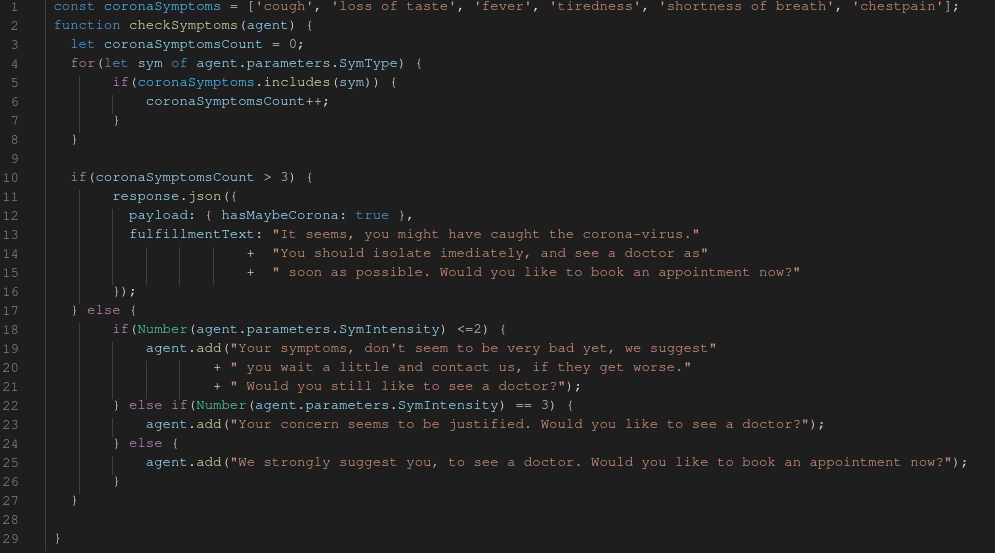
\includegraphics[width=\linewidth]{ressources/checkSymptoms.png}
            \end{center}
            \caption{checkSymptoms Funktion}
            \label{fig:checksymptomsfunction}
        \end{figure}
        \paragraph{}
            Auf den Zeilen 3 bis 8 werden die angegebenen Symptome mit dem Array \emph{coronaSymptoms} verglichen und gezählt.
            Auf Zeile 10 wird überprüft, ob die Anzahl der auf Corona-Symptome passenden Symptome grösser als 3 Ist. Ist dies
            der Fall wird unabhängig der anderen Parameter eine Entsprechende Nachricht zurückgesanddt, welche den Benutzer überprüft
            diesen Umstand informiert, und ihm vorschlägt, sich zu isolieren und testen zu lassen.

        \paragraph{}
            Besteht kein verdacht auf das Corona-Virus, so ist die Symtomstärke ("symtom\_intensity") Ausschlaggebend für die Antwort:
            \begin{itemize}
                \item Intensität kleiner oder gleich 2: Die Symptome scheinen nicht schlimm zu sein. Dem Benutzer wird geraten abzuwarten und bei
                    verschlimmerung des zustands einen Arzt aufzusuchen. Der Benutzer wird gefragt ob er dennoch einen Arzttermin buchen
                    möchte
                \item Intensität = 3: Der Benutzer wird gefragt, ob er einen Arzttermin buchen möchte.
                \item Intensität grösser 3: Dem Benutzer wird angeraten einen Arzt aufzusuchen. Er wird gefragt, ob er einen entsprechenden Termin
                    buchen möchte.
            \end{itemize}

        \paragraph{}
            Alle Antworten, fragen den Benutzer, ob er einen Arzttermin buchen will. Mit den Intents \emph{check\_symptoms - yes} und \emph{check\_symptoms - no}
            (Siehe: \ref{fig:intentslist}) wird die Antwort des Benutzers abgefangen. Während \emph{check\_symptoms - no} zu einer verabschiedungsantwort führt,
            fragt \emph{check\_symptoms - yes} direkt, danach wann der Termin gerne Stattfinden würde.

    \subsection{Termin buchen}
        \paragraph{}
            Der Intent \emph{check\_symptoms - yes - time} fängt die Antwort des vorgehenden Intents (Frage nach Terminzeit) direkt ab und löst im Webhook
            eine weitere Methode aus.
        \begin{figure}[h!]
            \begin{center}
                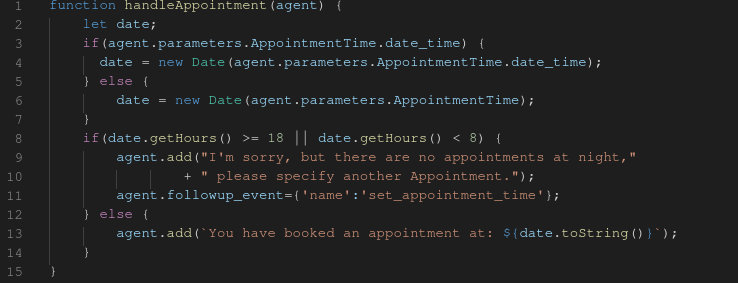
\includegraphics[width=0.7\linewidth]{ressources/handleAppointmentFunction.png}
            \end{center}
            \caption{handleAppointment Funktion}
            \label{fig:handleappointmentfunction}
        \end{figure}

        \paragraph{}
            Die ersten 7 Zeilen der Funktion kümmern sich um das Parsen des Datums. Da dieses nicht immer gleich daher kommt,
            musste ein wenig logik, zur überprüfung der Daten implementiert werden. Zeile 8 prüft, ob die Uhrzeit zwischen 08:00
            und 20:00 liegt. Alles zwischen diesen zwei Zeitpunkten ist als Gültige Uhrzeit definiert, und führt dazu dass die
            Buchung auf Zeile 13 Bestätigt wird. Der Dialog ist hiermit beendet. Liegt die Zeit allerdings ausserhalb des gültigen
            bereichs, wird auf den Zeilen 9 und 10 eine Fehlernachricht zurückgegeben und nach einer neuen Zeit gefragt.
            Auf Zeile 11 wird als folgeintent das Event \emph{set\_appointment\_time} definiert. Dieses Event zeit auf denselben 
            Intent, auf dem wir gerade operieren (\emph{check\_symptoms - yes -time}). Dies führt dazu das eine Logikschlaufe für 
            die Terminbuchung entsteht, bis eine gültige Zeit angegeben wird.

        \begin{figure}[h!]
            \begin{center}
                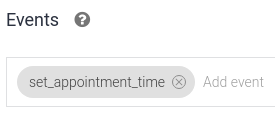
\includegraphics[width=0.4\linewidth]{ressources/eventSetting.png}
            \end{center}
            \caption{Eventeinstellung für die Schleiflogik}
            \label{fig:eventSetting}
        \end{figure}

        
\newpage

\section{Discussion}


\end{document} 